\documentclass[a4paper,14pt]{extreport}

\usepackage[T1,T2A]{fontenc}
\usepackage[utf8]{inputenc}

\usepackage{title}
\usepackage{bsumain}
\usepackage{blindtext}

\usepackage{hyperref}
\usepackage{subfigure}
\usepackage[final]{graphicx}

\title{Анализ эффективности нейросетевых вычислений с учетом аппаратных возможностей платформ}
\author{Бинцаровского Леонида Петровича}
\mentor{старший преподаватель\\
        Д. И. Пирштук}

\renewcommand\contentsname{Оглавление}

\begin{document}
    \maketitle\newpage
    
    \chapter*{Реферат}
    Курсовая работа, 36 стр., 2 иллюстр., 4 источника.\\
    \textbf{Ключевые слова:} Visual Studio; C++; Onnxruntime; DirectML; QNN; oneDNN; openVINO; DefaultCPU; инференс.\\
    \textbf{Объекты исследования} — анализ эффективности нейросетевых вычислений с учетом аппаратных возможностей платформ.\\
    \textbf{Цель исследования} — реализация классов для инференсов в среде разработки Visual Studio с целью сравнения эффективности нейросетевых вычеслений с учетом аппаратных возможностей платформ.\\
    \textbf{Методы исследования} — системный подход, изучение соответствующей литературы и электронных источников, постановка задачи и её решение.\\
    \textbf{В результате исследования} были реализованы классы на языке программирования с++ для инференса нейросетей в среде разработки Visual Studio. Проведены сравнения эффективности нейросетевых вычеслений с учетом аппаратных возможностей платформ.\\
    \textbf{Области применения} — инференс нейроных сетей.
    
    \tableofcontents\newpage
    \chapter*{Введение}
    \addcontentsline{toc}{chapter}{Введение}
    Нейронные сети стали неотъемлемой частью современного мира, найдя применение в самых разнообразных областях, начиная от компьютерного зрения и обработки естественного языка, и заканчивая медицинской диагностикой и финансовым анализом. С развитием глубокого обучения и доступностью вычислительных ресурсов, нейронные сети становятся все более распространенными и мощными инструментами для решения сложных задач, которые ранее казались невозможными или непрактичными для автоматизации. 

    Всвязи с постоянным увеличением объема данных и сложности задач, стоящих перед нейронными сетями, вопрос эффективности и скорости их работы становится все более актуальным. Одним из ключевых аспектов, определяющих производительность нейросетевых моделей, является скорость инференса - процесса получения выводов от модели на основе входных данных.

    \chapter{Постановка задачи}
    На данный момент существует огромное количество моделей предназначенных под всевозможные цели: улучшение качества изображения, перевод изображения из черно-белого в цветное, распознование речи и перевод ее в текст, сегментация объектов, перевод текста на разные языки и т.д. В рамках работы будут протестированы модели для semantic segmentation (разделение изображения на два класса: 1 -- объект, 0 -- фон), такие как mediapipe, selfie\_segmentation, SINet\_Softmax\_simple, rvm\_mobilentv3\_fp32 и pphumanseg\_fp32. Все вышеперечисленные модели имеют разную архитектуру, что в свою очередь влияет на скорость инференса. Также скорость инференса очень сильно зависит от используемых инструментов. Например, можно разворачивать модели только на базовых фреймворках — PyTorch, TensorFlow, PaddlePaddle, TFLite, TorchScript — и получать не самые лучшие результаты. Такие инструменты больше подходят для обучения и тестового инференса моделей, когда нет потребности в высокой скорости ML-сервиса. Для эффективной работы нужно использовать более мощные фреймворки, такие как ONNX Runtime, OpenVINO или TVM.
    
    Итак, сформулируем задачу анализа эффективности нейросетевых вычислений с учетом аппаратных возможностей платформ, которая будет изучаться в этой работе. Необходимо реализовать классы для инференса выбранной модели. На вход будет предоставлено изображение, на выходе - получена маска этого изображения и замерено время инференса. Затем, основываясь на полученных данных, будет проведена сравнительная характеристика провайдеров, которые были задействованы для инференса.

    \chapter{Обзор фреймворка ONNX Runtime}
        \section{Знакомство с ONNX Runtime}
        ONNX (Open Neural Network Exchange) - библиотека, реализующая хранение и обработку нейросетей, изначально называлась Toffe и разрабатывалась командой Pytorch (Meta). В 2017 проект был переименован в ONNX, и с тех пор поддерживается совместно Microsoft, Meta и другими большими компаниями.
        
        Изначально ONNX задумывался как открытый формат представления нейросети, который свяжет представление моделей в разных фреймворках.
        
        В первом релизе речь шла о Caffe2, PyTorch и CNTK. Сейчас многие крупные фреймворки стараются его поддерживать:

        \begin{figure}[h]
            \center{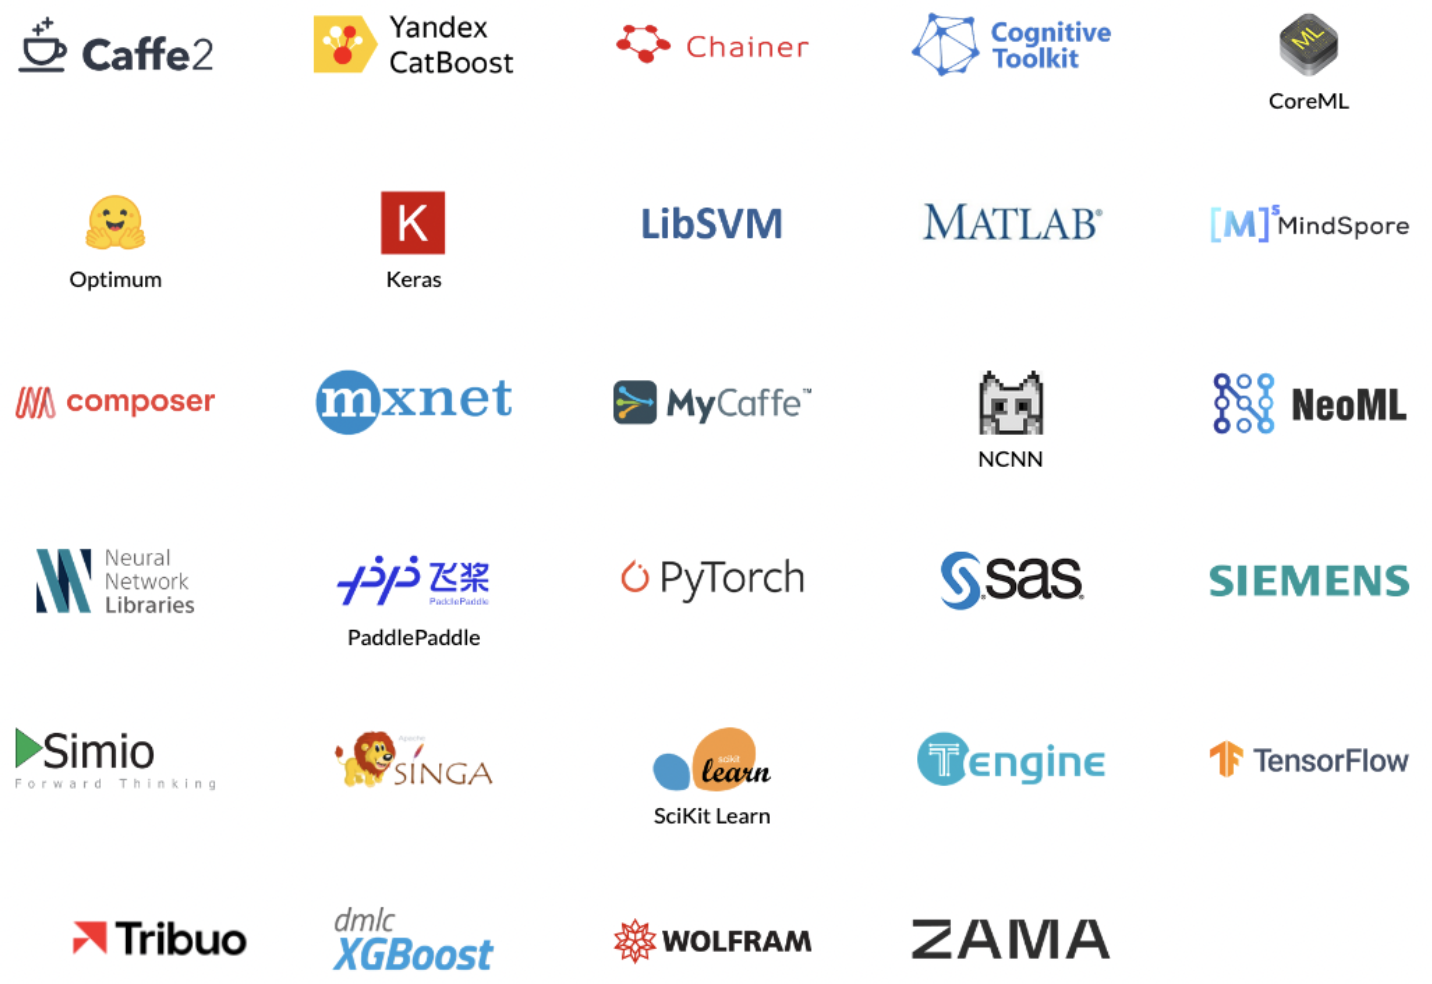
\includegraphics[width=1\linewidth]{images-onnxruntime/support.png}}
            \caption{Фреймворки, поддерживаемые ONNX Runtime}
            \label{ris:onnxruntime}
        \end{figure}

        Внутри у ONNX есть свое промежуточное представление. Оно реализовано с помощью protocol buffers и служит промежуточным звеном для конвертации между фреймворками. Все компоненты ONNX, включая промежуточное представление, версионируются возрастающим числом или согласно SemVer.
        
        Функции и операторы версионируются отдельно, а версия ONNX фиксируется в сериализуемой в protobuf модели.
        
        Это дает гарантию, что представление любой модели, даже спустя время, будет конвертироваться между ONNX и другими форматами. Иначе было бы легко запутаться при обновлении зависимостей в инфраструктуре.

        Через некоторое время появился ONNX Runtime - фреймворк для инференса в формате ONNX, который реализовал различные оптимизаторы поверх ONNX формата. Среди них ONNX Runtime DirectML, ONNX Runtime CoreML, ONNX Runtime TensorRT, ONNX Runtime CUDA, ONNX Runtime oneDNN, ONNX Runtime OpenVINO, ONNX Runtime QNN и т.д.

        \section{Конвертация моделей в формат ONNX}
        Для использования вышеперечисленных моделей (mediapipe.tflite, selfie\_segmentation.tflite, pphumaseg\_fp32.tflite, SINet\_softmax\_simple.tflite, rvm\_mobilnetv3\_fp32.tflite), их необходимо перевести из формата tflite в формат onnx. Для этого воспользуемся скриптом на python:
        \lstinputlisting[caption={Скрипт для конвертации tflite модели в onnx}]{codeOnnxruntime/converter.py}

        В данном скрипте используется фреймворк tf2onnx, предоставленный на официальном сайте ONNX Runtime. При использовании рукописного преобразователя могут возникнуть проблемы, так как не все слои конвертируются в ONNX формат. Часть может преобразоваться совсем не так как хотелось бы, а часть после конвертации может начать некорректно вычислять значения.

        \hypertarget{loader}{}Для удобства дальнейшего использования готового инференса, модели были загружены в h файлы. При использовании такого подхода, готовое приложение будет статически зависеть от модели и ее не нужно будет прикреплять к exe модулю. Для записи модели в массив был написан python скрипт:
        \lstinputlisting[caption={Скрипт для записи модели в массив char}]{codeOnnxruntime/loader.py}

    \chapter{Реализация кросс-платформенной части приложения для замера скорости вычислений нейросетей на языке С++}
        \section{Структура ORTModelData}
        Структура ORTModelData представляет собой контейнер, содержащий данные, необходимые для работы с моделью, которая загружена с использованием библиотеки ONNX Runtime (ORT).
        \lstinputlisting[language=c++, caption={Структура ORTModelData}]{codeORTModel/ORTModel.h}

        В структуре ORTModelData определены поля:
        \begin{itemize}
          \item[-] \textbf{session} — это уникальный указатель на объект сеанса Ort::Session, который является основным для выполнения модели. Сеанс содержит информацию о модели, включая ее граф вычислений, параметры и контекст выполнения. Он используется для загрузки и выполнения модели;
          \item[-] \textbf{env} — уникальный указатель на объект окружения Ort::Env. Ort::Env представляет собой контекст выполнения ONNX Runtime, содержит ресурсы и параметры, необходимые для работы с библиотекой ONNX Runtime;
          \item[-] \hypertarget{inputNames}{}\textbf{inputNames} — вектор указателей на строки Ort::AllocatedStringPtr, содержащих имена входных тензоров модели. Эти имена используются для связывания входных данных с соответствующими тензорами модели во время выполнения инференса;
          \item[-] \textbf{outputNames} — подобно \hyperlink{inputNames}{inputNames}, это вектор указателей на строки Ort::AllocatedStringPtr, содержащих имена выходных тензоров модели. Используются для извлечения выходных данных из соответствующих тензоров модели после выполнения инференса;
          \item[-] \textbf{inputTensor} — вектор объектов тензора Ort::Value, представляющих входные данные модели. Эти объекты тензора содержат входные данные, которые будут переданы в модель для инференса;
          \item[-] \textbf{outputTensor} — вектор объектов тензора Ort::Value, представляющих выходные данные модели. После выполнения модели, результаты будут содержаться в этих объектах тензора;
          \item[-] \hypertarget{inputDims}{}\textbf{inputDims} — вектор векторов целых чисел (int64\_t), содержащих размерности входных тензоров. Эти размерности определяют форму (shape) входных тензоров модели;
          \item[-] \textbf{outputDims} — аналогично \hyperlink{inputDims}{inputDims}, это вектор векторов целых чисел (int\_64t), содержащих размерности выходных тензоров модели;
          \item[-] \textbf{inputTensorValues} — вектор векторов чисел с плавающей запятой (float), содержащих значения входных тензоров модели. Эти значения представляют входные данные, которые будут переданы в модель для инференса;
          \item[-] \textbf{outputTensorValues} — вектор векторов чисел с плавающей запятой (float), содержащих значения выходных тензоров модели. Эти значения представляют собой результаты инференса модели;
        \end{itemize}

        \section{Классы Model и ModelBCHW}
        Для реализации класса Model была создана вспомогательная функция \textbf{vectorProduct}. Она принимает на вход вектор любого типа и возвращает произведение всех положительных элементов, так как 0 или -1 обычно обозначают "None".
        \lstinputlisting[language=c++, caption={Вспомогательная функция vectorProduct}]{codeModel/vectorProduct.cpp}
        
        Далее был реализован базовый класс для всех моделей - Model. Учитывалось, что все модели имеют один вход и один выход. На вход модели поступает 4D тензор формы (1, H, W, C), где H и W - высота и ширина входного изображения, С - количество цветовых каналов. Обычно цветные изображения используют 3 канала: красного, зеленого и синего цветов. Входные данные представлены в формате BGR и их диапозон - [0, 255]. Цель данного класса состоит в том, чтобы предоставить общий интерфейс для работы с моделями машинного обучения, которые обрабатывают изображения. 
        \lstinputlisting[language=c++, caption={Класс Model}]{codeModel/Model.h}

        В данном классе реализованны базовые методы для инференса. В последствии некоторые методы будут изменены в классах конкретных моделей.

        Метод \hypertarget{populateNames}{}\textbf{populateInputOutputNames} заполняет векторы inputNames и outputNames именами входных и выходных тензоров соответственно. В дальнейшем эти имена используются для запуска инференса модели.
        \lstinputlisting[language=c++, caption={Метод populateInputOutputNames}]{codeModel/populateOutput.cpp}

        Метод \hypertarget{populateShapes}{}\textbf{populateInputOutputShapes} заполняет векторы inputDims и outputDims размерностями входных и выходных тензоров соответственно. Он также выполняет проверку и корректировку размерностей, устанавливая любые отрицательные значения в размерности тензоров равными 1.
        \lstinputlisting[language=c++, caption={Метод populateInputOutputShapes}]{codeModel/populateInput.cpp}

        Метод \hypertarget{allocate}{}\textbf{allocateTensorBuffers} выделяет память для буферов входных и выходных тензоров и создает для них объекты Ort::Value.
        \lstinputlisting[language=c++, caption={Метод allocateTensorBuffers}]{codeModel/allocateBuffers.cpp}

        Метод \hypertarget{getSize}{}\textbf{getNetworkInputSize} получает размер входного изображения (ширину и высоту) из размерностей входного тензора.

        Метод \textbf{prepareInputToNetwork} выполняет предварительную обработку входного изображения перед передачей его в сеть. В данном случае он нормализует значения пикселей изображения в диапазоне от 0 до 1.

        Метод \hypertarget{postprocess}{}\textbf{postprocessOutput} выполняет постобработку выходных данных сети. Здесь он не выполняет никакой обработки, но будет переопределен в классах конкретных моделей для выполнения соотвествующей постобработки.

        Метод \textbf{loadInputToTensor} загружает предобработанное изображение во входной тензор модели.

        Метод \hypertarget{getOutput}{}\textbf{getNetworkOutput} получает выходные данные сети и возвращает их в виде объекта cv::Mat.
        
        Метод \hypertarget{assign}{}\textbf{assignOutputToInput} присваивает выходные данные входному тензору для обратной передачи в сеть. В данном случае он не выполняет никакой обработки, но будет переопределен в классах конкретных моделей для присваивания соответсвующих данных.

        Метод \hypertarget{runInference}{}\textbf{runNetworkInference} является ключевым для запуска модели на входных данных и получения выходных данных. Он позволяет использовать один и тот же общий интерфейс для выполнения инференса различных моделей и управления входными и выходными данными.
        \lstinputlisting[language=c++, caption={Метод runNetworkInference}]{codeModel/runNetwork.cpp}

        Для реализации класса ModelBCHW были реализованы вспомогательные функции.
        Функция \hypertarget{hwc_to_chw}{}\textbf{hwc\_to\_chw} преобразует входное изображение из формата HWC (высота x ширина x количество каналов) в формат CHW (количество каналов x высота x ширина).
        \lstinputlisting[language=c++, caption={Вспомогательная функция hwc\_to\_chw}]{codeModel/hwc_to_chw.cpp}

        Функция \hypertarget{chw_to_hwc_32f}{}\textbf{chw\_to\_hwc\_32f} преобразует изображение из формата CHW (количество каналов x высота x ширина) в формат HWC (высота x ширина x количество каналов) для изображений с плавающей точкой (float32).
        \lstinputlisting[language=c++, caption={Вспомогательная функция chw\_to\_hwc\_32f}]{codeModel/chw_to_hwc_32f.cpp}

        Далее был реализован сам класс ModelBCHW. Он является наследником базового класса Model и представляет собой специализированную версию модели, которая работает с данными в формате BCHW (количество каналов x высота x ширина).
        \lstinputlisting[language=c++, caption={Метод runNetworkInference}]{codeModel/ModelBCHW.h}

        Метод \textbf{prepareInputToNetwork} выполняет предварительную обработку входного изображения перед передачей его в сеть. Он нормализует значения пикселей изображения в диапазоне от 0 до 1 и затем преобразует изображение из формата HWC в формат BCHW с помощью функции \hyperlink{hwc_to_chw}{hwc\_to\_chw}.

        Метод \textbf{postprocessOutput} выполняет постобработку выходных данных сети. Он транспонирует изображение из формата BCHW обратно в формат HWC с помощью функции \hyperlink{chw_to_hwc_32f}{chw\_to\_hwc\_32f}, чтобы его можно было корректно отобразить или использовать дальше.

        Метод \textbf{getNetworkInputSize} получает размер входного изображения (ширину и высоту) из размерностей входного тензора в формате BCHW.
        
        Метод \textbf{getNetworkOutput} получает выходные данные сети и возвращает их в виде объекта cv::Mat в формате HWC.
        
        Метод \textbf{loadInputToTensor} загружает предобработанное изображение во входной тензор модели. Он копирует значения пикселей изображения в одномерный вектор входного тензора.
        
        \section{Структуа FilterData}
        Эта структура предназначена для хранения основных данных, необходимых для фильтров ORT (ONNX Runtime). FilterData наследует все поля, определенные в структуре ORTModelData, так как она должна иметь доступ к базовым данным модели ORT. 
        \lstinputlisting[language=c++, caption={Структура FilterData}]{codeFilterData/FilterData.h}

        Непосредственно в структуре FilterData определены поля:
        \begin{itemize}
          \item[-] \textbf{useGPU} — строка, содержащая информацию о том, какой провайдер использовать. Может быть установлен флаг CPU, DirectML, QNN, oneDNN или OpenVINO;
          \item[-] \textbf{numThreads} — переменная, определяющая количество потоков, используемых для выполнения инференса;
          \item[-] \textbf{modelSelection} — строка, содержащая название модели, которая будет использоваться для обработки данных;
          \item[-] \textbf{model} — Уникальный указатель на объект модели, который будет использоваться для выполнения инференса;
          \item[-] \textbf{inputBGRA} — матрица изображения (cv::Mat) в формате BGRA (синий, зеленый, красный, альфа), которая будет подаваться на вход модели;
          \item[-] \textbf{inputBGRALock} — объект мьютекса для безопасного доступа к входным данным;
          \item[-] \textbf{modelInfo} и \textbf{modelSize} — указатель на информацию о модели и ее размер, которые будут использованы для хранения информации о модели;
        \end{itemize}

        \section{Класс ModelMediapipe}
        Класс \textbf{ModelMediapipe} является производным от базового класса Model. Он предназначен для работы непосредственно с моделью mediapipe. Так как модель mediapipe возвращает тензор размерности (B, H, W, C) и изображение с двумя каналами (0 - маска фона, 1 - маска человека), необходимо переопределить методы \hyperlink{getOutput}{getNetworkOutput} и \hyperlink{postprocess}{postprocessOutput}.
        \lstinputlisting[language=c++, caption={Класс ModelMediapipe}]{codeModelClasses/ModelMediapipe.h}

        \section{Класс ModelPPHumanseg}
        Класс \textbf{ModelPPHumanseg} является производным от класса ModelBCHW. Он предназначен для работы с моделью pphumanseg\_fp32. Так как модель pphumanseg\_fp32 принимает на вход тензор BCHW, возвращает тензор размерности (B, H, W, C) и изображение с двумя каналами (0 - маска фона, 1 - маска человека), необходимо переопределить методы \hyperlink{prepareInput}{prepareInputToNetwork}, \hyperlink{getOutput}{getNetworkOutput} и \hyperlink{postprocess}{postprocessOutput}.
        \lstinputlisting[language=c++, caption={Класс ModelPPHumanseg}]{codeModelClasses/ModelPPHumanseg.h}

        \section{Класс ModelSelfie}
        Класс \textbf{ModelSelfie} является производным от класса Model. Он предназначен для работы с моделью selfie\_segmentation. Для этого необходимо переопределить лишь метод \hyperlink{postprocess}{postprocessOutput}.
        \lstinputlisting[language=c++, caption={Класс ModelSelfie}]{codeModelClasses/ModelSelfie.h}

        \section{Класс ModelSINET}
        Класс \textbf{ModelSINET} является производным от класса ModelBCHW. Он предназначен для работы с моделью SINet\_softmax\_simple. Для этого необходимо переопределить лишь метод \hyperlink{prepareInput}{prepareInputToNetwork}, так как модель SINet\_softmax\_simple принимает на вход тензор BCHW.
        \lstinputlisting[language=c++, caption={Класс ModelSINET}]{codeModelClasses/ModelSINET.h}

        \section{Функции createOrtSession и runFilterModelInference}
        Так как модели были преобразованы в ONNX, а \hyperlink{loader}{затем записаны в массив char}, необходимо подключить нужный хедер. Для этого были установлены макросы, определяющие какая именно модель необходима для текущего инференса:
        \lstinputlisting[language=c++, caption={Подключение необходимых хедеров для функции createOrtSession}]{codeOrtSessionUtils/includes.h}

        Функция \hypertarget{createOrt}{}\textbf{createOrtSession} реализована, чтобы создать сеанс для выполнения инференса конкретной модели. 
        
        Изначально проверяется задана ли модель. Если нет -- возвращается ошибка, и инференс останавливается. Затем задаются настройки параметров сеанса. В зависимости от текущей модели, задаются modelInfo и modelSize. Далее устанавливается текущий провайдер. Это может быть DirectML, OpenVINO, QNN или oneDNN. Если ни один из них не установлен, инференс будет происходить на CPU. Если для инференса используется CPU -- устанавливается заданное число используемых ядер CPU. Далее создается новая сессия для модели c использованием указанных параметров, информации о ней и опции сеанса. Если при создании сеанса возникает ошибка -- выводится сообщение об ней. Далее для созданной модели вызываются методы \hyperlink{populateNames}{populateInputOutputNames}, \hyperlink{populateShapes}{populateInputOutputShapes} и \hyperlink{allocate}{allocateTensorBuffers}.
        \lstinputlisting[language=c++, caption={Вспомогательная функция createOrtSession}]{codeOrtSessionUtils/createOrtSession.cpp}

        Функция \hypertarget{runFilter}{}\textbf{runFilterModelInference} используется для выполнения инференса модели с применением сеанса, который был предварительно создан в \hyperlink{createOrt}{createOrtSession}, и подготовленных в структуре FilterData данных. Сначала идет проверка того, что сеанс ONNX Runtime и объект модели инициализированы и готовы к использованию. Если нет -- функция возвращает false и выводит сообщение об ошибке. Если они инициализированы -- изображение изменяется до размера, ожидаемого входными данными модели, с использованием cv::resize. Размер определяется методом \hyperlink{getSize}{getNetworkInputSize}. Затем подготовленное изображение преобразуется в формат, который ожидает модель и загружается в объект тензора для передачи в сеанс выполнения. Выполняется инференс модели с помощью метода \hyperlink{runInference}{runNetworkInference}. После выполнения инференса данные преобразуются в формат cv::Mat с использованием метода \hyperlink{getOutput}{getNetworkOutput}. При необходимоти результаты могут быть перенаправлены на входные данные для последующих итераций модели с помощью метода \hyperlink{assign}{assignOutputToInput}. Вывод модели обрабатывается с помощью метода \hyperlink{postprocess}{postprocessOutput} и конвертируется в формат CV\_8U (8-битное изображение) для дальнейшего использования.
        \lstinputlisting[language=c++, caption={Вспомогательная функция runFilterModelInference}]{codeOrtSessionUtils/runFilterModelInference.cpp}

        \section{Класс BackgroundFilter}
        Класс \textbf{BackgroundFilter} является связующим звеном. Именно в нем реализованы методы, в которые пользователь передает входные данные, может установить параметры для модели и сессии инференса.
        \lstinputlisting[language=c++, caption={Класс BackgroundFilter}]{codeBackgroundFilter/BackgroundFilter.h}

        В конструкторе данного класса инициализируется объект tf, который содержит базовую информацию для работы с ORT. Создается новая среда для работы с ORT, и ее уровень логирования устанавливается на уровень ошибок. Выбирается модель по умолчанию -- modiapipe.

        Метод \textbf{filterUpdateThreads} обновляет количество задействованных ядер CPU и устанавливает их в указанное значение.
        \lstinputlisting[language=c++, caption={Метод filterUpdateThreads}]{codeBackgroundFilter/Threads.cpp}

        Метод \textbf{filterUpdateModel} устанавливает текущую модель для инференса. По умолчанию модель инициализируется как модель mediapipe. На вход принимает строку с названием модели для инференса.
        \lstinputlisting[language=c++, caption={Метод filterUpdateModel}]{codeBackgroundFilter/Model.cpp}

        Метод \textbf{filterUpdateProvider} устанавливает текущий провайдер. По умолчанию установлен провайдер CPU от ONNXRuntime. 
        \lstinputlisting[language=c++, caption={Метод filterUpdateProvider}]{codeBackgroundFilter/Provider.cpp}

        Метод \hypertarget{defines}{}\textbf{setDefines} устанавливает макрос текущей модели. В дальнейшем данный макрос будет использован в функции \hyperlink{createOrt}{createOrtSession} для загрузки необходимой модели в память.

        Метод \textbf{filterActivateChanges} устанавливает макрос для текущей модели при помощи функции \hyperlink{defines}{setDefines} и, если сессия не создана (флаг initialized == false), создает ее с помощью функции \hyperlink{createOrt}{createOrtSession}.

        Метод \textbf{getMask} возвращает текущую маску для входного изображения.

        Метод \textbf{setInputImage} устанавливает поле tf->inputRGB. Для этого в данный метод передается размерность изображения (высота x ширина), тип входного изображения и его данные. В методе создается временный cv::Mat для преобразования типа из BGR в RGB. Затем блокируется мьютекс inputRGBLock с помощью std::lock\_guard, и при помощи std::move перемещаются данные из tempRGB в tf->inputRGB. Таким образом удается минимизировать накладные расходы на копирование данных.
        \lstinputlisting[language=c++, caption={Метод setInputImage}]{codeBackgroundFilter/SetInputImage.cpp}

        Метод \textbf{filterVideoTick} обрабатывает входное изображение и возвращает маску в поле tf->backgroundMask. Метод начинается с проверки входного изображения. Если оно пустое -- метод заканчивает работу и выдает ошибку. Далее изображение извлекается из tf->inputRGBLock, чтобы предотвратить возможный одновременный доступ к нему. Если все выполнилось успешно -- изображение передается на инференс модели. Для этого используется вспомогательная функция \hyperlink{imageForBackground}{processImageForBackground}. Если на каком-то из этапов инференса происходит ошибка, она выводится, и работа метода завершается.
        \lstinputlisting[language=c++, caption={Метод filterVideoTick}]{codeBackgroundFilter/filterVideoTick.cpp}

        Метод \hypertarget{imageForBackground}{}\textbf{processImageForBackground} запускает инференс модели фильтра. Для этого вызывается функция \hyperlink{runFilter}{runFilterModelInference}, в которой выполняется инференс модели фильтра на входном изображении и возвращает результат в переменной outputImage. Если инференс не удался -- метод завершается. \lstinputlisting[language=c++, caption={Метод processImageForBackground}]{codeBackgroundFilter/processImageForBackground.cpp}
    
    \chapter{Тестирование фреймворков}
        \section{Реализация тестовой программы}
        Для тестирования работы инференса была реализована программа, в которой реализовано два основных цикла. Первый цикл предназначен для "разогрева" модели. Для большей точности были замерены результаты "разогрева" на 100, 200 и 300 итерациях. Второй цикл работал в основном режиме. Замеры были проведены на 3000 итерациях инференса. В обоих случаях на вход модели предоставлялось изображение:
        \begin{figure}[h]
            \center{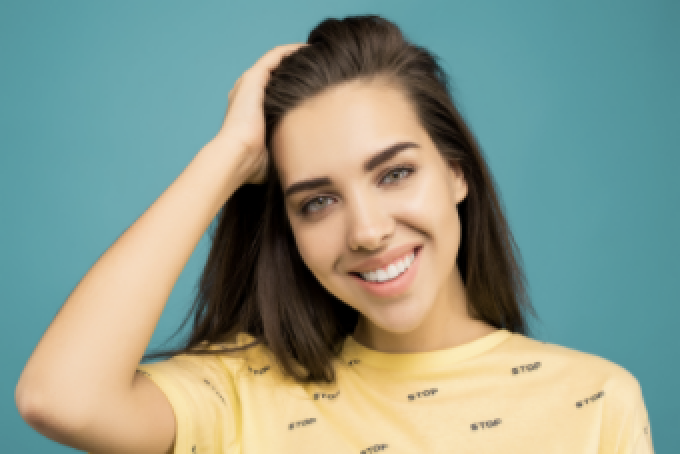
\includegraphics[width=0.49\linewidth]{images-program/input.png}}
            \caption{Входное изображение}
            \label{ris:input}
        \end{figure}
        
        Ниже представлен код для тестирования инференса модели pphumnseg\_fp32 на провайдере OpenVINO с использованием 1 ядра CPU:
        \lstinputlisting[language=c++, caption={Код тестирующей программы}]{codeTesting/testingProgram.cpp}

        \section{Анализ результатов}
        При тестировании инференса модели замерялось максимальное, минимальное и среднее время выполнения. Результаты измерялись в миллисекундах. Замеры производились на разных провайдерах: DefaultCPU, OpenVINO, QNN, DirectML и oneDNN. При использовании провайдера DefaultCPU были измерены зависимости скорости инференса от разного количества задействованных ядер CPU: 1 и 3.

        В данной таблице представлены результаты инференса модели mediapipe:
        \begin{table}[htbp]
            \centering
            \begin{tabular}{|c|c|c|}
                \hline
                \textbf{"Разогрев"} & \textbf{100} & \textbf{300} \\
                \hline
                QNN & Min:6ms & Min:5ms\\
                    & Max:18ms & Max:11ms\\
                    & Average:6ms & Average:6ms\\
                \hline
                DirectML & Min:7ms & Min:6ms\\
                         & Max:17ms & Max:14ms\\
                         & Average:7ms & Average:6ms\\
                \hline
                OpenVINO & Min:8ms & Min:8ms\\
                         & Max:38ms & Max:43ms\\
                         & Average:9ms & Average:8ms\\
                \hline
                oneDNN & Min:10ms & Min:9ms\\
                       & Max:58ms & Max:45ms\\
                       & Average:12ms & Average:11ms\\
                \hline
                DefaultCPU & Min:11ms & Min:11ms\\
                1 ядро     & Max:40ms & Max:47ms\\
                           & Average:11ms & Average:11ms\\
                \hline
                DefaultCPU & Min:7ms & Min:7ms\\
                3 ядра     & Max:54ms & Max:33ms\\
                           & Average:8ms & Average:9ms\\
                \hline
            \end{tabular}
            \caption{Результаты инференса модели mediapipe}
            \label{tab:exampleQNN}
        \end{table}

        Тесты всех провайдеров, кроме DirectML, проводились на Macbook с чипом M1. Для этого была установлена виртуальная машина windows 11, при помощи программы Parallels Desktop. Тестирование провайдера DirectML пришлось проводить на стороннем устройстве, так как виртуальная машина windows 11 не могла получить доступ к GPU.

        Из приведенных таблиц видно, что при обработке на DefaultCPU, от количества используемых ядер меньше всего зависят модели mediapipe и selfie\_segmentation. При разработке данных моделей учитывалось, что они будут использоваться на мобильных устройствах, поэтому они и демонстрируют такие результаты, независимо от количества задействованных ядер CPU.

        \begin{figure}[!h]
            \begin{center}
                \begin{minipage}[h]{0.4\linewidth}
                    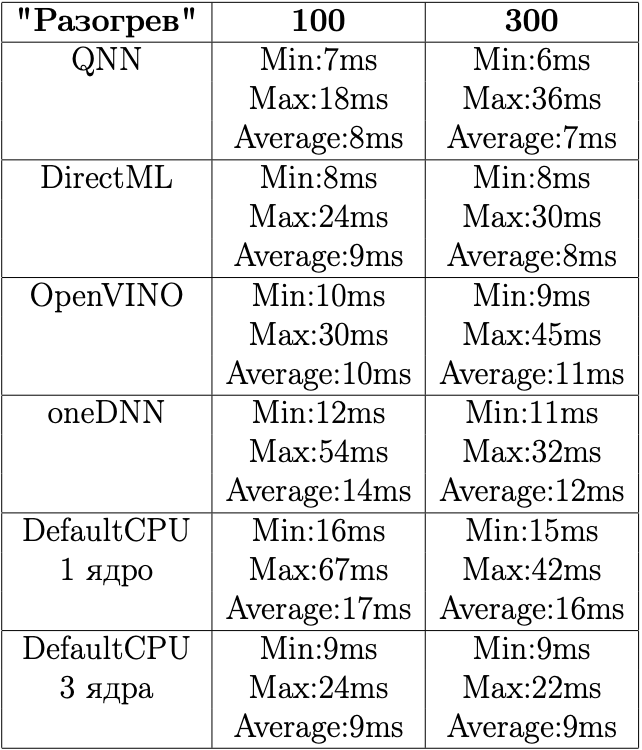
\includegraphics[width=1\linewidth]{images-results/selfie.png}
                    \caption{Инференс selfie\_segmentation}
                    \label{ris:selfie}
                \end{minipage}
                \hfill
                \begin{minipage}[h]{0.4\linewidth}
                    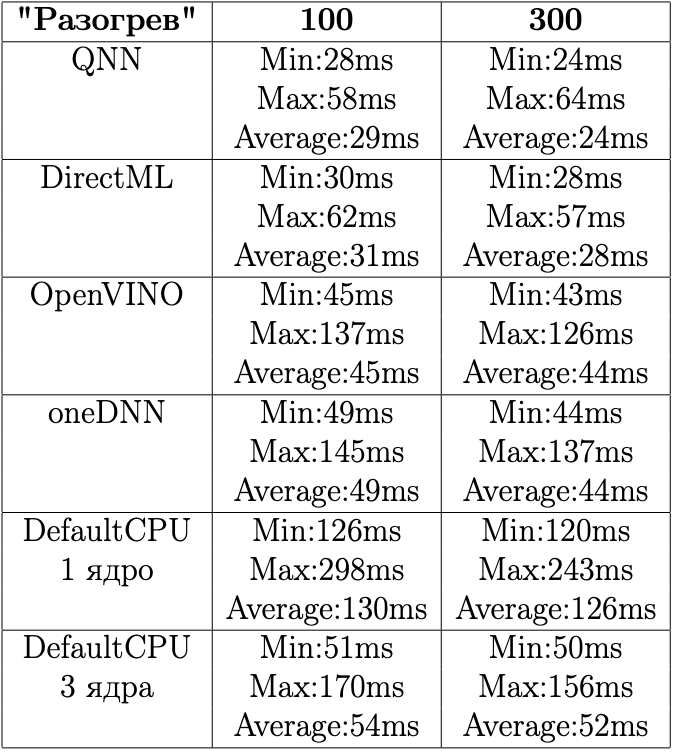
\includegraphics[width=1\linewidth]{images-results/rvm.png}
                    \caption{Инференс rvm\_mobilenetv3\_fp32}
                    \label{ris:rvm}
                \end{minipage}
            \end{center}
        \end{figure}
        
        \begin{figure}[!h]
            \begin{center}
                \begin{minipage}[h]{0.4\linewidth}
                    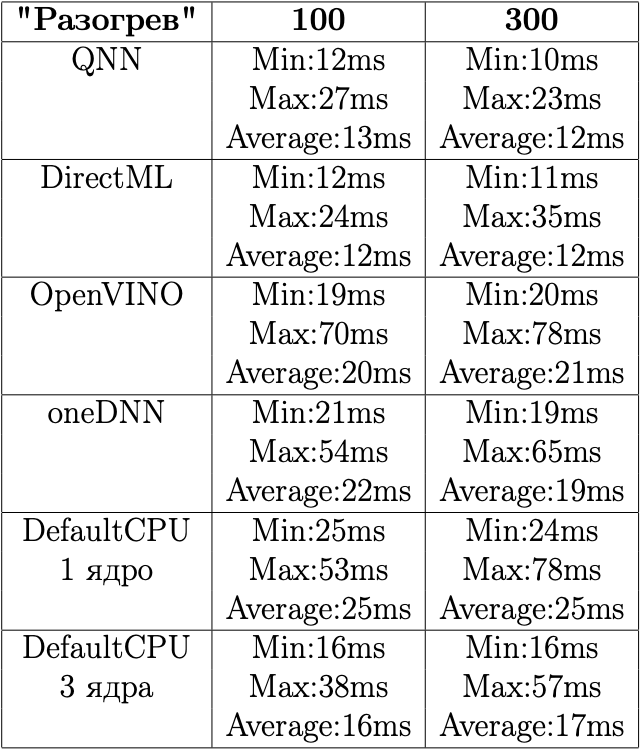
\includegraphics[width=1\linewidth]{images-results/sinet.png}
                    \caption{Инференс SINet\_softmax\_simple}
                    \label{ris:sinet}
                \end{minipage}
                \hfill
                \begin{minipage}[h]{0.4\linewidth}
                    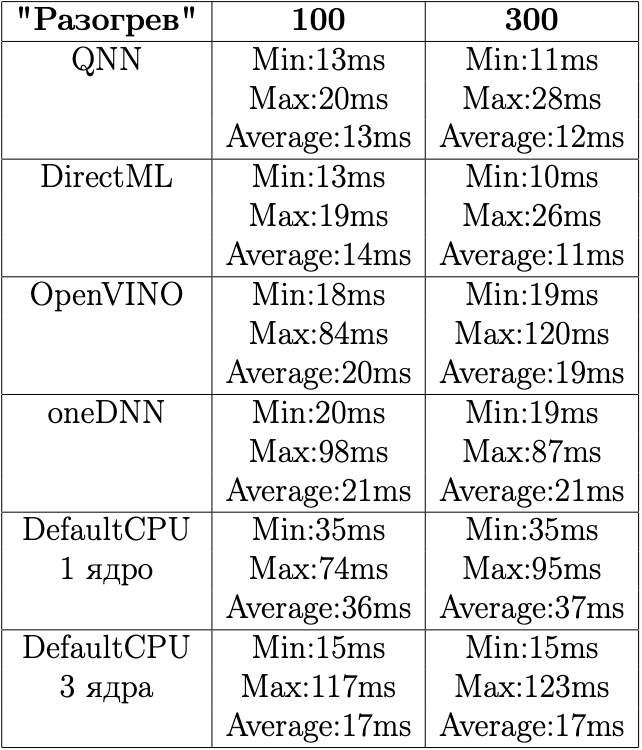
\includegraphics[width=1\linewidth]{images-results/pphumaseg.png}
                    \caption{Инференс pphumanseg\_fp32}
                    \label{ris:pphumanseg}
                \end{minipage}
            \end{center}
        \end{figure}

        По итогу тестирования, лучшими провайдерами оказались QNN и DirectML. Они на всех тестируемых моделях показали лучший результат, в некоторых случаях с большим отрывом от других провайдеров (рис. \ref{ris:rvm}). Это связано с архитектурой процессора, под который проектировался провайдер QNN: ARM. Что же касается DirectML -- это единственный провайдер, который был реализован на GPU, из-за чего он и тестировался на стороннем компьютере.
        
        Следующими по скорости инференса для моделей mediapipe (таблица \ref{tab:exampleQNN}) и  rvm\_mobilenetv3\_fp32 (рис. \ref{ris:rvm}) стали результаты провайдера OpenVINO. Для остальных моделей -- Default CPU с использованием 3 ядер. Хотелось бы отметить, что при такой конфигурации (DefaultCPU, 3 ядра) было задействовано приблизительно 80\% CPU. Провайдер OpenVINO разрабатывался Intel и существенный прирост производительности отмечается имеено на их процессорах. В связи с чем OpenVINO и продемонстрировал результат сопоставимый с DefaultCPU, 3 ядра. 

        Последним по скорости инференса всех моделей стал провайдер DefaultCPU с использованием 1 ядра. В некоторых случаях результат работы данного провайдера был сравним с работой oneDNN (таблица \ref{tab:exampleQNN}, рис. \ref{ris:sinet}), но в большинстве своем сильно уступал. При использовании модели rvm\_mobilenetv3\_fp32 скорость инференса на провайдере DefaultCPU (1 ядро) была почти в 4 раза медленнее чем на провайдере QNN.

    \chapter*{Заключение}
    \addcontentsline{toc}{chapter}{Заключение}
    В ходе курсовой работы:
    \begin{enumerate}
        \item Сделан краткий обзор фреймворка ONNX Runtime и провайдеров OpenVINO, DirectML, oneDNN, QNN и DefaultCPU;
        \item Реализованы классы для кросс-платформенного инференса моделей mediapipe, Selfie\_segmentation, pphumanseg\_fp32, SINet\_softmax\_simple и rvm\_mobilenetv3\_fp32; 
        \item Реализованы платформозависимые компоненты: DirectML, OpenVINO, oneDNN, QNN;
        \item Создана тестовая программа для замера скорости инференса выбранной модели;
        \item Проведено сравнение скорости инференса моделей в зависимости от используемого провайдера или количеста ядер CPU.
    \end{enumerate}

    \chapter*{Список использованных источников}
    \addcontentsline{toc}{chapter}{Список использованных источников}
    \begin{enumerate}
        \item Qualcomm Technologies, Inc. (2024). Qualcomm Neural Processing SDK for Windows on Snapdragon [Электронный ресурс]: Qualcomm Developer Network. Режим доступа: \href{https://developer.qualcomm.com/software/qualcomm-neural-processing-sdk/wi ndows-on-snapdragon}{https://developer.qualcomm.com/software/qualcomm-neural-processing-sdk/wi ndows-on-snapdragon}. Дата доступа: 15.05.2024
        \item ONNX Runtime Execution Providers [Электронный ресурс]: ONNX Runtime. – Redmond, WA: Microsoft Corporation, 2021. – Режим доступа: \href{https://onnxruntime.ai/docs/execution-providers/}{https://onnxruntime.ai/docs/execution-providers/}. Дата доступа: 15.05.2024
        \item Ashfaq, S., AskariHemmat, M., Sah, S., Saboori, E., Mastropietro, O., \& Hoffman, A. (2022). Accelerating Deep Learning Model Inference on Arm CPUs with Ultra-Low Bit Quantization and Runtime [Электронный ресурс]: Deeplite Inc. – Montreal, Canada: Deeplite Inc., 2022. – Режим доступа: \href{https://arxiv.org/pdf/2207.08820.pdf}{https://arxiv.org/pdf/2207.08820.pdf}. Дата доступа: 15.05.2024
        \item Lee, J., Chirkov, N., Ignasheva, E., Pisarchyk, Y., Shieh, M., Riccardi, F., Sarokin, R., Kulik, A., \& Grundmann, M. (2019). On-Device Neural Net Inference with Mobile GPUs [Электронный ресурс]: Google Research. – Режим доступа: \href{https://ar5iv.labs.arxiv.org/html/1907.01989}{https://ar5iv.labs.arxiv.org/html/1907.01989}. Дата доступа: 15.05.2024

    \end{enumerate}
    
\end{document}
